\documentclass{beamer}
\usepackage{animate}
\usepackage{tikz}
\usetheme{Madrid}
\useinnertheme{circles}
%Information to be included in the title page:
\title{A Gentle Introduction to (Large) Language Models}
\subtitle{From word2vec to ChatGPT}
\author{Jakub Koubele}
\institute{Beyer lab retreat}
\date{22nd August, 2025}

\renewcommand{\insertshortauthor}{Jakub Koubele}  
\renewcommand{\insertshorttitle}{An Introduction to LLMs}
\renewcommand{\insertshortdate}{22nd August, 2025} % Define custom text for 3rd block

\graphicspath{{./figures/}}

\usepackage{amsthm}
\newcommand*{\QED}{\hfill\ensuremath{\blacksquare}}





\begin{document}
	\frame{\titlepage}
	


\begin{frame}
	\frametitle{What is a language, anyway?}
	\pause
	\begin{tikzpicture}[remember picture,overlay]
		\node at (1.9cm, -2.3cm) {\includegraphics[scale=0.16]{gutten_morgen}};
	\end{tikzpicture}

	\begin{tikzpicture}[remember picture,overlay]
		\node at (4.0cm, 2.1cm) {\includegraphics[scale=0.17]{hobbit}};
	\end{tikzpicture}

	\begin{tikzpicture}[remember picture,overlay]
		\node at (8.0cm, -2.05cm) {\includegraphics[scale=0.105]{doom_sqrt_2}};
	\end{tikzpicture}

	\begin{tikzpicture}[remember picture,overlay]
		\node at (9.9cm, 2.4cm) {\includegraphics[scale=0.105]{green_ideas}};
	\end{tikzpicture}



\end{frame}
	
	
\begin{frame}
	\frametitle{Tokenization}
	\pause
	\begin{itemize}
		\item Text = sequence of symbols.
		\item Alphabet = set of all symbols.
		
		\pause
		\item Symbol can be represented by one-hot vector.
		\begin{tikzpicture}[remember picture,overlay]
			\node at (2.0cm, 0.4cm) {\includegraphics[scale=0.21]{one_hot}};
		\end{tikzpicture}
		
		\pause 
		\item Which alphabet we should use?
		\begin{itemize}
			\item Words?
			\item Letters?			
		\end{itemize}
	\pause
	\item Subword tokenization (e.g., WordPiece) is commonly used.
	
	\begin{tikzpicture}[remember picture,overlay]
		\node at (5.2cm, -0.35cm) {\includegraphics[scale=0.22]{tokenizer}};
	\end{tikzpicture}	
		
	\end{itemize}
\end{frame}

\begin{frame}
	\frametitle{Problems of one-hot encoding}
	\pause
	\begin{itemize}
		\item After tokenization, we have a sequence of tokens, represented by one-hot vectors.
		\begin{center}
			\includegraphics[scale=0.18]{one_hot_sequence}		
		\end{center}
	\pause	
	\item Problems:
	\begin{itemize}		
		\item High dimensionality (alphabet size usually 10k - 100k symbols).
		\item Spare vectors without much information.
		
	\end{itemize}
		
	\end{itemize}
\end{frame}
	
	
\begin{frame}
	\frametitle{Distributed word representation}
	\pause
	\begin{columns}[T] % [T] aligns content at the top
		\begin{column}{0.8\textwidth}
			\begin{itemize}
				\item We would like to represent the tokens (words) by vectors that:
				\begin{itemize}
					\item Are dense, with reasonable dimensionality (e.g., 100~–~500).		
					\begin{tikzpicture}[remember picture,overlay]
						\node at (7.8cm, 0.40cm) {\includegraphics[scale=0.17]{dense}};						
					\end{tikzpicture}	
					\pause 			
					\item Arithmetic of these vectors (addition, subtraction etc.) 
					captures the semantics of words.
				\end{itemize}
			\end{itemize}				
		
		\end{column}
		\begin{column}{0.20\textwidth}			
		\end{column}	
	\end{columns}
\begin{center}
	\includegraphics[scale=0.13]{pca_combined}		
\end{center}
\end{frame}

\begin{frame}
	\frametitle{Word2vec (2013)}
	\pause
	
	\begin{itemize}
		\item Two similar models, predicting word(s) from vector representation of words nearby. The vectors are parameters of the model, and are learned by maximum likelihood estimation (MLE).
	\end{itemize}
	\begin{center}
		\includegraphics[scale=0.10]{word2vec}		
	\end{center}

\begin{tikzpicture}[remember picture,overlay]
	\node at (5.7cm, -0.37cm) {\includegraphics[scale=0.10]{banking}};
\end{tikzpicture}	
	
\end{frame}

\begin{frame}
	\frametitle{Brief intro to neural networks}
	\pause
	\begin{columns}[T] % [T] aligns content at the top
		\begin{column}{0.8\textwidth}
	\begin{itemize}
		\item Neural networks are \textbf{functions}, that...
		\pause 
		\begin{itemize}
			\item Work with \textbf{tensors} (nd-arrays).
			\pause 
			\item Are \textbf{compound} (composite of simple operations).
			
			\begin{itemize}
				\item May be represented by directed acyclic \textbf{computational graph}.				
			\end{itemize}
		
		\begin{tikzpicture}[remember picture,overlay]
			\node at (9.1cm, 1.2cm) {\includegraphics[scale=0.14]{comp_graph}};
		\end{tikzpicture}
	
		\pause 
		\item Are \textbf{parametrized}.
		\pause 
		\item Are \textbf{differentiable} (loss of output with respect to the parameters).		
		\begin{itemize}
			\item Parameters are learned by gradient methods.			
		\end{itemize}
			
		\end{itemize}
	\end{itemize}

	\end{column}
	\begin{column}{0.20\textwidth}			
	\end{column}	
	\end{columns}
	
\end{frame}


\begin{frame}
	\frametitle{Recurrent neural networks (RNNs)}
	\pause
	\begin{columns}[T] % [T] aligns content at the top
		\begin{column}{0.75\textwidth}
	\begin{itemize}
		\item RNNs are specialized for sequential data. 
		\pause 
		\item Have \textbf{inner state} that is passed through time.
		
		\begin{itemize}
		\item Output depends on the inner state.
		\item Taking input updates the inner state.		
		\end{itemize}
	
	\begin{center}
		\includegraphics[scale=0.20]{rnn}		
	\end{center}
	\pause		
	\item Many different architectures, most popular \\ one  is the Long-Short Term Memory (LSTM).
	\end{itemize}
\begin{tikzpicture}[remember picture,overlay]
	\node at (10.45cm, 1.77cm) {\includegraphics[scale=0.17]{lstm}};
\end{tikzpicture}

\end{column}
\begin{column}{0.25\textwidth}			
\end{column}	
\end{columns}
	
	
\end{frame}

\begin{frame}
	\frametitle{Google Translator (2016)}
	\pause
	\begin{tikzpicture}[remember picture,overlay]
		\node at (5.75cm, -0.95cm) {\includegraphics[scale=0.16]{google_translator}};
	\end{tikzpicture}

	\begin{tikzpicture}[remember picture,overlay]
	\node at (8.65cm, 3.25cm) {\includegraphics[scale=0.12]{liebe_dich}};
\end{tikzpicture}


\end{frame}

\begin{frame}
	\frametitle{All you need is...}
	\pause
	\begin{columns}[T] % [T] aligns content at the top
		\begin{column}{0.85\textwidth}
	\begin{itemize}
		\item Before 2017, the best performing model architectures were based on LSTM.
		\pause
		\item Until...they weren't.
		\pause
		\begin{center}
			\includegraphics[scale=0.13]{attention_paper}		
		\end{center}
		
	\end{itemize}

\end{column}
\begin{column}{0.15\textwidth}			
\end{column}	
\end{columns}

\pause
\begin{tikzpicture}[remember picture,overlay]
	\node at (10.2cm, 2.75cm) {\includegraphics[scale=0.125]{transformer_architecture}};
\end{tikzpicture}


\end{frame}

\begin{frame}
	\frametitle{Attention layer}
	\pause


\begin{tikzpicture}[remember picture,overlay]
	\node at (5.85cm, 0.35cm) {\includegraphics[scale=0.23]{attention_layer}};
\end{tikzpicture}

\begin{tikzpicture}[remember picture,overlay]
	\node at (6.85cm, -2.55cm) {\includegraphics[scale=0.3]{attention_formula}};
\end{tikzpicture}
	
\end{frame}


\begin{frame}
	\frametitle{Attention visualization}
	\pause
	
	\begin{tikzpicture}[remember picture,overlay]
		\node at (5.85cm, -0.05cm) {\includegraphics[scale=0.11]{attention_visualization}};
	\end{tikzpicture}

	\begin{tikzpicture}[remember picture,overlay]
		\node at (6.05cm, -3.3cm) {\includegraphics[scale=0.24]{fig_text}};
	\end{tikzpicture}



\end{frame}

\begin{frame}

\frametitle{BERT (Bidirectional Encoder Representation from Transformer)}

	\begin{tikzpicture}[remember picture,overlay]
	\node at (11.65cm, -5.6cm) {\includegraphics[scale=0.15]{bert}};
\end{tikzpicture}

\pause
\begin{itemize}
	\item Pre-train transformer on masked-word prediction.
	\begin{itemize}
		\item No labeled data needed, can be done on large corpus.		
	\end{itemize}
	\pause
	\item Finetune on task-specific labeled data.	
\end{itemize}

\pause

	\begin{center}
	\includegraphics[scale=0.13]{bert_architecture}		
\end{center}

\end{frame}

\begin{frame}	
	
	\frametitle{GPT (Generative Pretrained Transformer)}
	\pause
	\begin{itemize}
		\item Pretrained on next word prediction.
		\pause
		\item Worse performance than BERT for fine-tunning, but good for  generating text.
		\pause
		\item Few-shot / zero-shot learning without gradient updates.
		
			\begin{center}
			\includegraphics[scale=0.20]{few_shot}		
		\end{center}
		
		
	\end{itemize}
	
\end{frame}

\begin{frame}
	\frametitle{Generating text is not enough}
	\pause
		\begin{center}
		\includegraphics[scale=0.18]{instruct_gpt}		
	\end{center}
	
\end{frame}
	
\begin{frame}	
	
	\frametitle{Reinforcement Learning from Human Feedback (RLHF)}
	\pause
	\begin{center}
		\includegraphics[scale=0.163]{rlhf}		
	\end{center}
\end{frame}

\begin{frame}	
	
	\frametitle{The End}
	Thanks for your attention! (It's all you need).
	
	\begin{center}
		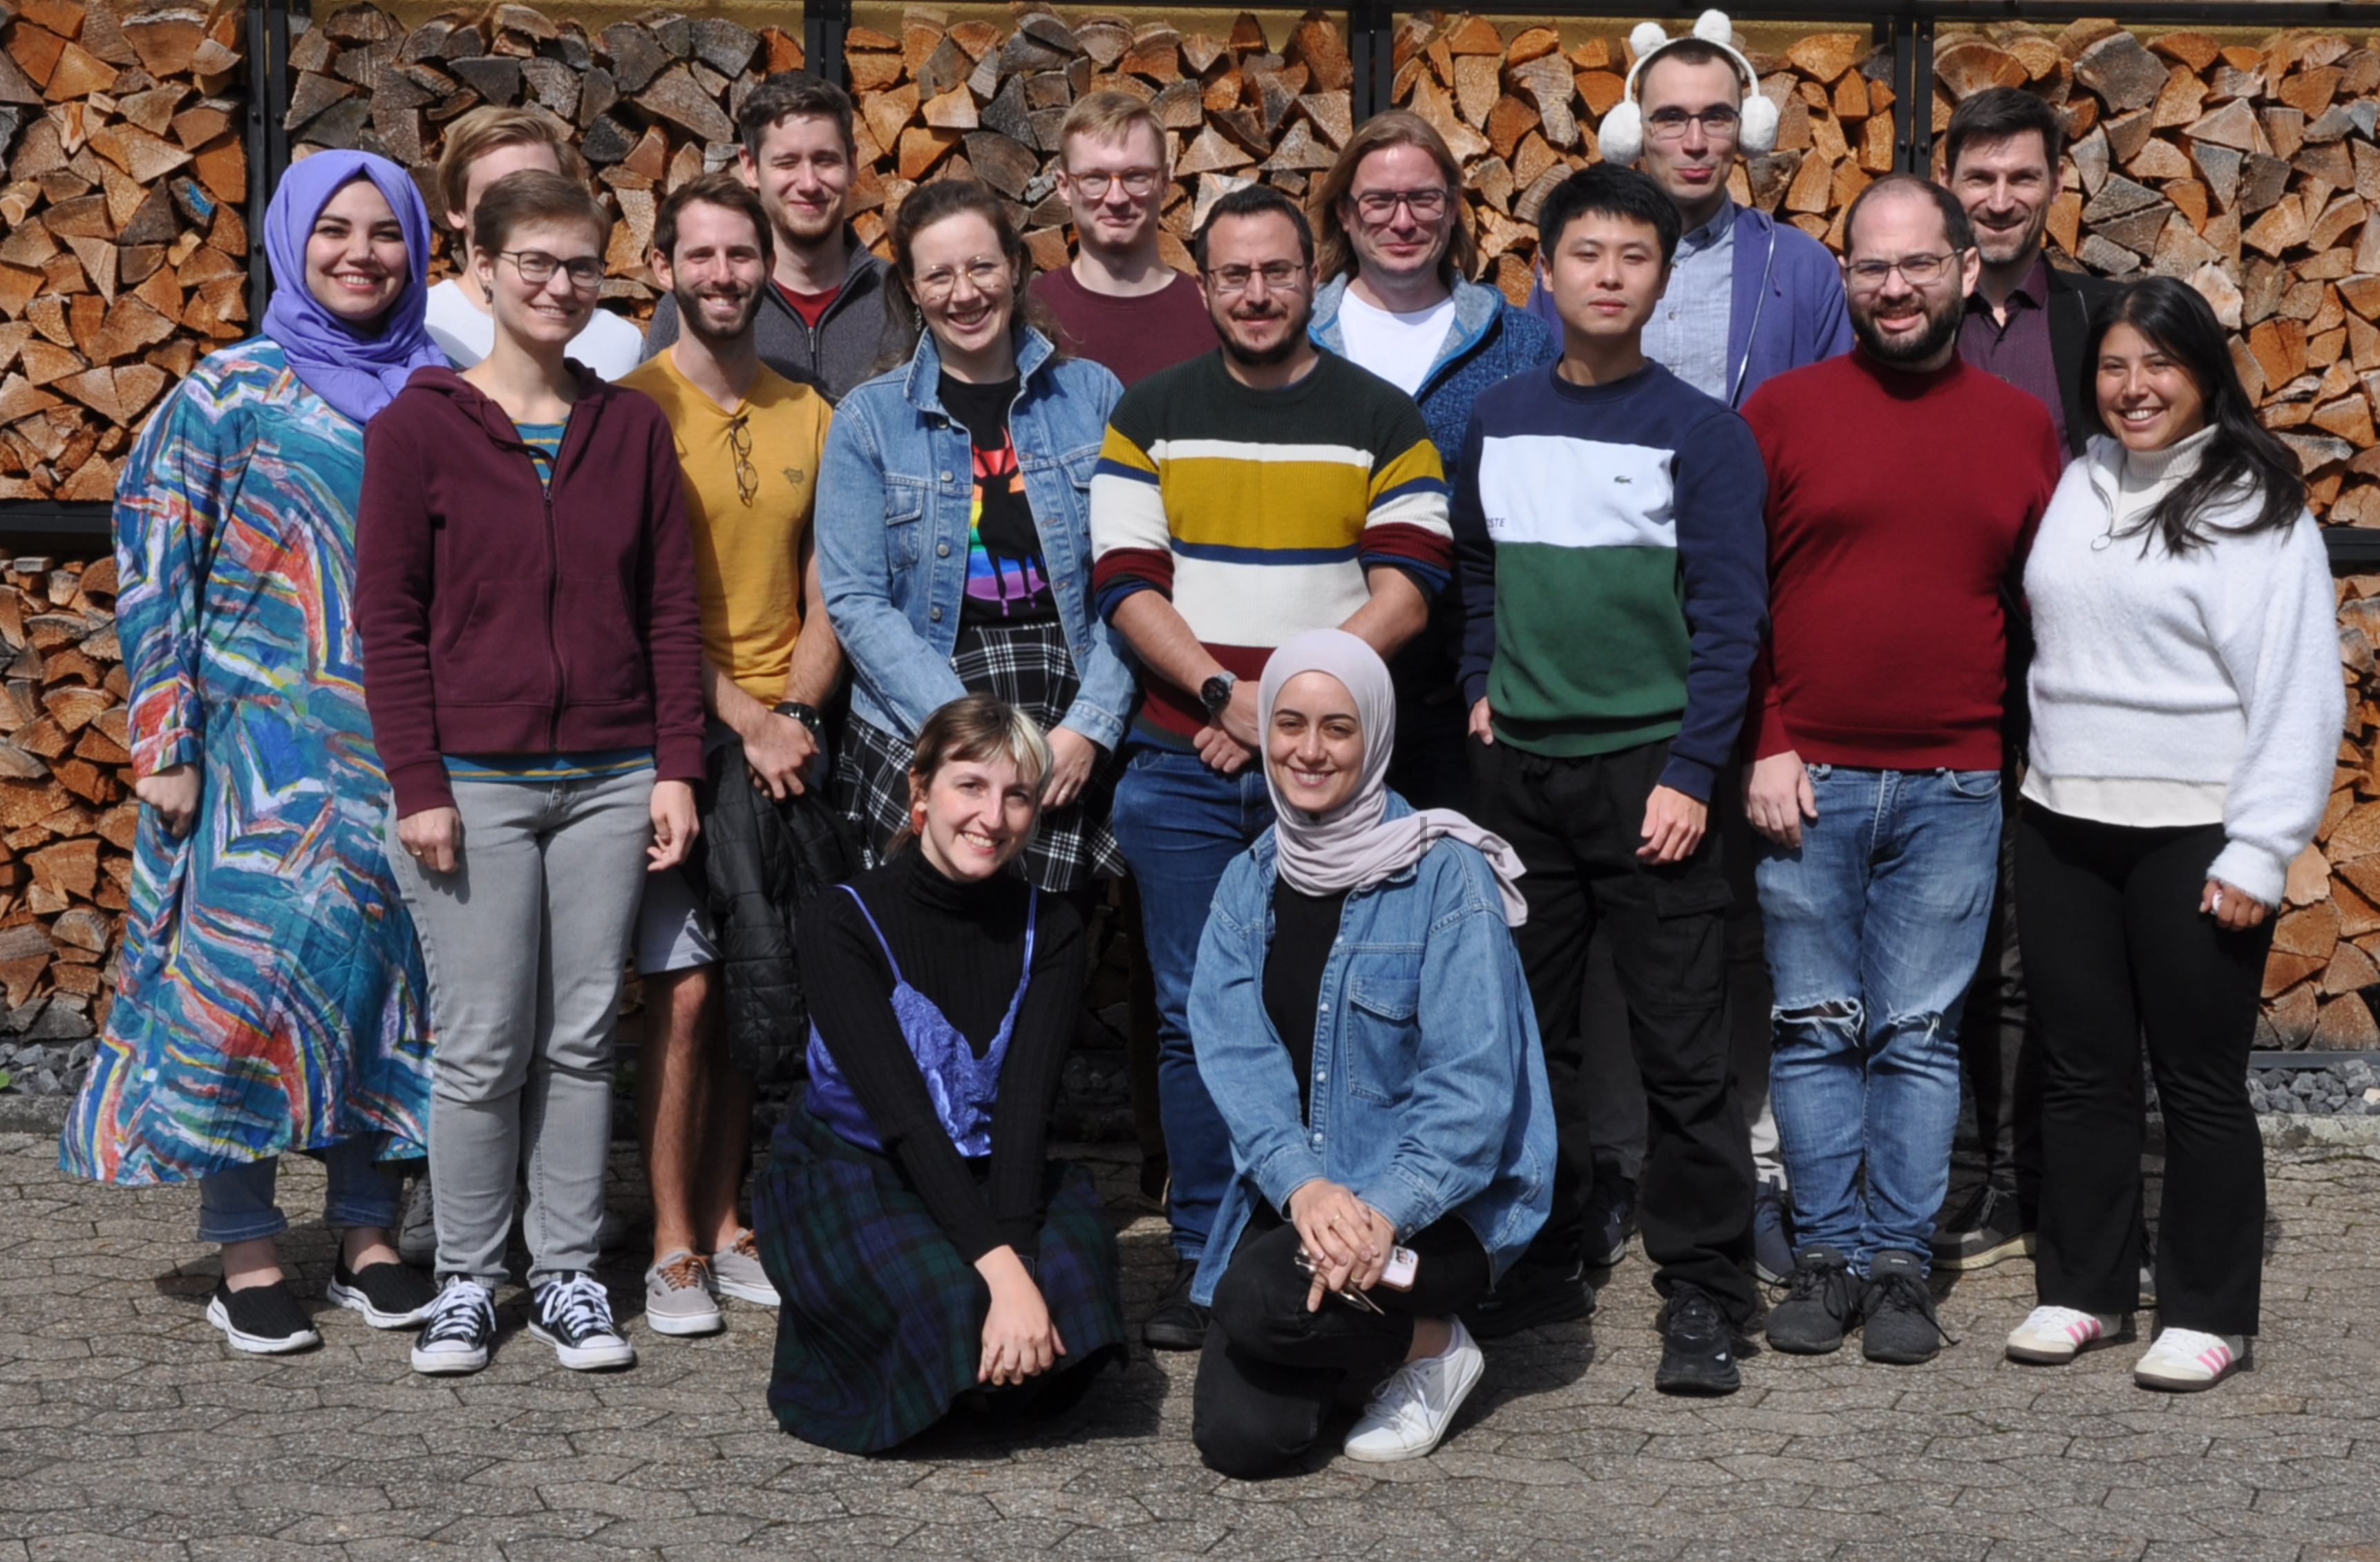
\includegraphics[scale=0.083]{group_picture}		
	\end{center}
\end{frame}

\begin{frame}
	\frametitle{References (1/2)}
	{\footnotesize
	\textbf{General references}
	\begin{itemize}
		\item \href{https://www.deeplearningbook.org/}{Goodfellow, Ian, et al. Deep learning. (2016).}
		\item \href{https://github.com/huggingface/transformers}{Transformers library}
		\item \href{https://web.stanford.edu/class/archive/cs/cs224n/cs224n.1246/}{CS224N at Standford}		
	\end{itemize}
	\textbf{Papers (1/2)}
	\begin{itemize}
	\item Mikolov, Tomas, et al. "Efficient estimation of word representations in vector space." (2013).
	\item Mikolov, Tomas, et al. "Distributed representations of words and phrases and their compositionality." (2013).
	\item Pennington, Jeffrey, Richard Socher, and Christopher D. Manning. "Glove: Global vectors for word representation." (2014).
	\item Wu, Yonghui, et al. "Google's neural machine translation system: Bridging the gap between human and machine translation." (2016).
	\item Vaswani, Ashish, et al. "Attention is all you need." (2017).	
	


\end{itemize}
}
\end{frame}

\begin{frame}
	\frametitle{References (2/2)}
	
	{\footnotesize
		\textbf{Papers (2/2)}
		\begin{itemize}
			\item Devlin, Jacob, et al. "Bert: Pre-training of deep bidirectional transformers for language understanding." (2019).
			\item Radford, Alec, et al. "Improving language understanding by generative pre-training." (2018).
			\item Radford, Alec, et al. "Language models are unsupervised multitask learners." (2019)
			\item Brown, Tom, et al. "Language models are few-shot learners." (2020)
			\item Ouyang, Long, et al. "Training language models to follow instructions with human feedback." (2022).
		\end{itemize}
		
}

\end{frame}	


	
\end{document}
